% Gabarit pandoc des corrigés publiés (brut et guidé). Contenu sans marque ni nom de site.
% Compilation : lualatex (latexmk -lualatex).
% Le Markdown reste la source unique : ne pas éditer ce fichier .tex à la main.
\documentclass[11pt,a4paper]{article}

% --- Moteur, polices (Latin Modern) et langue ---------------------------------
\usepackage{iftex}
\ifLuaTeX\else\errmessage{Ce document se compile avec lualatex}\fi
\usepackage{amsmath,amssymb,mathtools}
\usepackage{fontspec}
% mathrm=sym : \mathrm prend ses glyphes dans la police mathématique (ℓ, μ, Ω), comme KaTeX.
\usepackage[math-style=TeX,bold-style=TeX,mathrm=sym]{unicode-math}
% Repli pour les glyphes absents de Latin Modern (indices et exposants Unicode,
% flèches, filets des schémas en texte, symboles) : DejaVu, puis Latin Modern Math
% (ℓ, lettres mathématiques Unicode des légendes).
\directlua{
  luaotfload.add_fallback("repliTexte", {"DejaVuSerif:mode=harf;", "DejaVuSans:mode=harf;", "file:latinmodern-math.otf:mode=harf;"})
  luaotfload.add_fallback("repliMono", {"DejaVuSansMono:mode=harf;", "DejaVuSans:mode=harf;", "file:latinmodern-math.otf:mode=harf;"})
}
\setmainfont{Latin Modern Roman}[RawFeature={fallback=repliTexte}]
\setsansfont{Latin Modern Sans}[RawFeature={fallback=repliTexte}]
\setmonofont{Latin Modern Mono}[RawFeature={fallback=repliMono}]
\setmathfont{Latin Modern Math}
\usepackage[french]{babel}
\frenchsetup{SmallCapsFigTabCaptions=false}

% --- Mise en page --------------------------------------------------------------
\usepackage[a4paper,margin=2.2cm,headheight=14pt,footskip=1.2cm]{geometry}
\usepackage{microtype}
\setlength{\emergencystretch}{4em}
\tolerance=1500
\setlength{\parindent}{0pt}
\setlength{\parskip}{0.55\baselineskip plus 2pt minus 1pt}
\usepackage{xcolor}
% Gris nommés : babel-french rend « ! » actif dans le document.
\definecolor{gris2}{gray}{0.98}
\definecolor{gris3}{gray}{0.97}
\definecolor{gris5}{gray}{0.95}
\definecolor{gris35}{gray}{0.65}
\definecolor{gris40}{gray}{0.60}
\definecolor{gris45}{gray}{0.55}
\definecolor{gris50}{gray}{0.50}
\definecolor{gris55}{gray}{0.45}
\definecolor{gris60}{gray}{0.40}
\definecolor{gris65}{gray}{0.35}
\definecolor{gris70}{gray}{0.30}
\definecolor{gris80}{gray}{0.20}
\definecolor{gris85}{gray}{0.15}
\usepackage{graphicx}
\usepackage{float}
\usepackage{caption}
\captionsetup{font=small,labelformat=empty,justification=centering}
\usepackage{booktabs,longtable,array,multirow,calc}
\usepackage{siunitx}
\sisetup{locale=FR}
\usepackage[version=4]{mhchem}
\usepackage{listings}
\usepackage{fancyhdr}
\usepackage{lastpage}
\usepackage[most]{tcolorbox}
\usepackage{enumitem}
\setlist{nosep,leftmargin=*,topsep=2pt}
\usepackage[hidelinks,unicode]{hyperref}
\usepackage{bookmark}
\hypersetup{pdftitle={CCINP PSI — Physique-chimie 2026},pdfauthor={Rédigé par IA},pdfcreator={LaTeX},pdfsubject={Corrigé brut}}
\usepackage{xurl}

% --- Pandoc : listes, tableaux, figures ----------------------------------------
\providecommand{\passthrough}[1]{#1}
\providecommand{\tightlist}{\setlength{\itemsep}{0pt}\setlength{\parskip}{0pt}}

\makeatletter
\def\maxwidth{\ifdim\Gin@nat@width>\linewidth\linewidth\else\Gin@nat@width\fi}
\def\maxheight{\ifdim\Gin@nat@height>0.55\textheight 0.55\textheight\else\Gin@nat@height\fi}
\makeatother
\setkeys{Gin}{width=\maxwidth,height=\maxheight,keepaspectratio}
\setcounter{secnumdepth}{-\maxdimen}
\providecommand{\pandocbounded}[1]{#1}

% --- Code (listings) -----------------------------------------------------------
\lstset{
  basicstyle=\ttfamily\small,
  columns=fullflexible,
  keepspaces=true,
  breaklines=true,
  breakatwhitespace=false,
  postbreak=\mbox{\textcolor{gris50}{$\hookrightarrow$}\space},
  frame=single,
  rulecolor=\color{gris35},
  framesep=4pt,
  xleftmargin=5pt,xrightmargin=5pt,
  backgroundcolor=\color{gris3},
  keywordstyle=\bfseries,
  commentstyle=\color{gris65},
  stringstyle=\color{gris80},
  showstringspaces=false,
  tabsize=4,
  extendedchars=true,
  aboveskip=6pt,belowskip=6pt,
}

% --- Macros des corrigés (KaTeX ↔ LaTeX) ---------------------------------------
% Les corrigés sont écrits pour KaTeX : on définit ici ce que KaTeX connaît et
% que LaTeX n'a pas, sans jamais retoucher le Markdown.
\providecommand{\R}{\mathbb{R}}
\providecommand{\N}{\mathbb{N}}
\providecommand{\Z}{\mathbb{Z}}
\providecommand{\Q}{\mathbb{Q}}
\providecommand{\C}{\mathbb{C}}
\providecommand{\dd}{\mathrm{d}}
\providecommand{\llbracket}{\lBrack}
\providecommand{\rrbracket}{\rBrack}
\providecommand{\lBrace}{\lbrace}
\providecommand{\rBrace}{\rbrace}
\providecommand{\Box}{\square}
\providecommand{\Diamond}{\lozenge}
\providecommand{\varnothing}{\emptyset}
\providecommand{\argmax}{\operatorname*{arg\,max}}
\providecommand{\argmin}{\operatorname*{arg\,min}}
\renewcommand{\leq}{\leqslant}
\renewcommand{\geq}{\geqslant}

% Équation hors texte : réduite à la largeur de la ligne si elle déborde.
\newsavebox{\boiteequation}
\newcommand{\equationajustee}[1]{%
  \sbox{\boiteequation}{$\displaystyle #1$}%
  \ifdim\wd\boiteequation>\linewidth
    \[\resizebox{\linewidth}{!}{\usebox{\boiteequation}}\]%
  \else
    \[#1\]%
  \fi}

% --- Encadrés pédagogiques (sobres, lisibles en noir et blanc) -----------------
\tcbset{
  encadre/.style={
    enhanced,breakable,sharp corners,
    colback=white,colframe=gris55,
    boxrule=0.4pt,leftrule=2.2pt,
    left=6pt,right=6pt,top=3pt,bottom=3pt,
    before skip=6pt,after skip=6pt,
    fonttitle=\bfseries\small,coltitle=black,
    attach title to upper,after title={\quad},
    parbox=false,
  }
}
\newtcolorbox{indication}[1]{encadre,colframe=gris45,colback=gris2,title={Indication~#1}}
\newtcolorbox{methode}{encadre,colframe=gris70,title={Méthode}}
\newtcolorbox{piege}{encadre,colframe=gris85,boxrule=0.8pt,leftrule=2.2pt,title={Piège}}
\newtcolorbox{jury}{encadre,colframe=gris60,colback=gris5,title={Jury}}
\newtcolorbox{encadrenote}{encadre,colframe=gris40}

% --- Titres de section ---------------------------------------------------------
\usepackage{titlesec}
\titleformat{\section}{\Large\bfseries}{}{0pt}{}
\titleformat{\subsection}{\large\bfseries}{}{0pt}{}
\titleformat{\subsubsection}{\normalsize\bfseries}{}{0pt}{}
\titlespacing*{\section}{0pt}{14pt plus 4pt minus 2pt}{6pt}
\titlespacing*{\subsection}{0pt}{10pt plus 3pt minus 2pt}{4pt}
\titlespacing*{\subsubsection}{0pt}{8pt plus 2pt minus 2pt}{2pt}

% --- En-tête et pied de page ---------------------------------------------------
\pagestyle{fancy}
\fancyhf{}
\fancyhead[L]{\small\textsc{Corrigé brut} · CCINP PSI}
\fancyhead[R]{\small Physique-chimie 2026}
\fancyfoot[L]{\footnotesize Corrigé rédigé par IA, non officiel}
\fancyfoot[R]{\footnotesize \thepage\,/\,\pageref*{LastPage}}
\renewcommand{\headrulewidth}{0.4pt}
\renewcommand{\footrulewidth}{0pt}
\fancypagestyle{plain}{\fancyhf{}\fancyfoot[R]{\footnotesize \thepage\,/\,\pageref*{LastPage}}\fancyfoot[L]{\footnotesize Corrigé rédigé par IA, non officiel}\renewcommand{\headrulewidth}{0pt}}

\begin{document}
\thispagestyle{plain}
\begin{center}
  {\small\scshape Corrigé brut}\par\smallskip
  {\LARGE\bfseries CCINP PSI — Physique-chimie 2026\par}\medskip
  {\large CCINP · PSI · Physique-chimie · 2026\par}
\end{center}
\vspace{2pt}\hrule\vspace{8pt}

\emph{Corrigé rédigé par IA, non officiel. Signalez toute erreur.}

Épreuve de 4 heures, calculatrices interdites. « Semi-conducteurs et convertisseurs de puissance », quatre parties indépendantes, 36 questions.

\hypertarget{partie-i-dopage-des-semi-conducteurs}{%
\section{Partie I --- Dopage des semi-conducteurs}\label{partie-i-dopage-des-semi-conducteurs}}

\hypertarget{q1}{%
\subsection{Q1}\label{q1}}

Loi de Fick : \(\vec\jmath=-D\,\overrightarrow{\mathrm{grad}}\,C\), soit à une dimension
\equationajustee{\boxed{j(x,t)=-D\,\frac{\partial C}{\partial x}(x,t)}}
Le signe \(-\) traduit le transport des zones concentrées vers les zones diluées.

Unités :

\begin{itemize}
\tightlist
\item
  \(C\), nombre d'atomes par unité de volume, en \(\mathrm{m^{-3}}\) ;
\item
  \(j\), nombre d'atomes traversant l'unité de surface par unité de temps, en \(\mathrm{m^{-2}\cdot s^{-1}}\) ;
\item
  par homogénéité, \([D]=[j][x]/[C]\), donc \(\boxed{D\ \text{en}\ \mathrm{m^2\cdot s^{-1}}}\).
\end{itemize}

\hypertarget{q2}{%
\subsection{Q2}\label{q2}}

Système : la tranche fixe de substrat comprise entre \(x\) et \(x+\mathrm dx\), de section droite \(S\) perpendiculaire à \((Ox)\). Elle contient \(N(t)=C(x,t)\,S\,\mathrm dx\) atomes de phosphore. La diffusion n'ayant lieu que selon \((Ox)\), aucun flux ne traverse les faces latérales.

\begin{figure}[H]
\centering
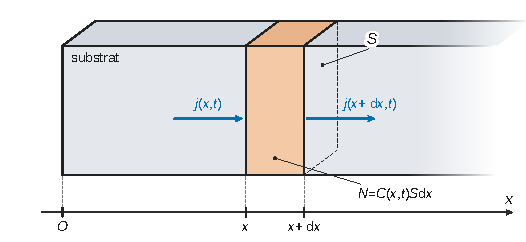
\includegraphics{figures/q02-bilan-tranche.pdf}
\caption*{Figure 1 --- Bilan sur la tranche fixe de substrat entre x et x + dx, de
section S : flux j(x, t) entrant, j(x + dx, t) sortant}
\end{figure}

Entre \(t\) et \(t+\mathrm dt\), il entre \(j(x,t)S\,\mathrm dt\) atomes par la face d'abscisse \(x\). Il en sort \(j(x+\mathrm dx,t)S\,\mathrm dt\) par la face d'abscisse \(x+\mathrm dx\). Sans création ni disparition d'atomes, la variation du nombre d'atomes de la tranche vaut :
\equationajustee{\begin{aligned}
N(t+\mathrm dt)-N(t)&=\frac{\partial C}{\partial t}S\,\mathrm dx\,\mathrm dt\\
&=\big[j(x,t)-j(x+\mathrm dx,t)\big]S\,\mathrm dt\\
&=-\frac{\partial j}{\partial x}S\,\mathrm dx\,\mathrm dt
\end{aligned}}
d'où
\equationajustee{\boxed{\frac{\partial C}{\partial t}+\frac{\partial j}{\partial x}=0}}

\hypertarget{q3}{%
\subsection{Q3}\label{q3}}

Le substrat est homogène, donc \(D\) est uniforme. En reportant la loi de Fick dans la relation de Q2 :
\equationajustee{\boxed{\frac{\partial C}{\partial t}=D\,\frac{\partial^2 C}{\partial x^2}}}
C'est l'équation de diffusion.

\hypertarget{q4}{%
\subsection{Q4}\label{q4}}

Les deux membres de l'équation ont pour ordres de grandeur \(C/\tau_c\) et \(DC/L_c^2\). En les égalant, avec des coefficients adimensionnés de l'ordre de l'unité :
\equationajustee{\boxed{L_c\sim\sqrt{D\,\tau_c}}}
soit \(\tau_c\sim L_c^2/D\). La longueur de diffusion croît comme la racine carrée de la durée : pour doubler la profondeur, il faut quadrupler la durée.

\hypertarget{q5}{%
\subsection{Q5}\label{q5}}

Le substrat occupe le demi-espace \(x>0\) (figure 1). Considérons un cylindre de substrat de section unité, d'axe \((Ox)\), appuyé sur le plan \(x=0\). Il contient \(\sigma\) atomes à \(t=0\).

Par conservation, il en contient encore \(\sigma\) pour tout \(t>0\), tous ayant diffusé dans le substrat :
\equationajustee{\int_0^{+\infty}C(x,t)\,\mathrm dx=\sigma .}
Avec \(u=x/(2\sqrt{Dt})\), on a \(\mathrm dx=2\sqrt{Dt}\,\mathrm du\), d'où :
\equationajustee{\begin{aligned}
\int_0^{+\infty}\frac{\alpha}{\sqrt t}e^{-x^2/(4Dt)}\,\mathrm dx&=\frac{\alpha}{\sqrt t}\,2\sqrt{Dt}\int_0^{+\infty}e^{-u^2}\,\mathrm du\\
&=\frac{\alpha}{\sqrt t}\,2\sqrt{Dt}\,\frac{\sqrt\pi}{2}\\
&=\alpha\sqrt{\pi D}
\end{aligned}}
Le résultat ne dépend pas de \(t\), ce qui confirme la cohérence de la solution admise. Donc
\equationajustee{\boxed{\alpha=\frac{\sigma}{\sqrt{\pi D}}}}
(\(\alpha\) en \(\mathrm{m^{-3}\cdot s^{1/2}}\), de sorte que \(\alpha/\sqrt t\) est bien une concentration.)

\hypertarget{q6}{%
\subsection{Q6}\label{q6}}

\(C(0,t)=\alpha/\sqrt t\), donc la définition de \(p\) s'écrit :
\equationajustee{\begin{aligned}
C(p,t)=\frac1e\,C(0,t)&\iff\exp\!\Big(-\frac{p^2}{4Dt}\Big)=e^{-1}\\
&\iff p^2=4Dt
\end{aligned}}
et, avec \(p>0\),
\equationajustee{\boxed{p=2\sqrt{Dt}}}
C'est cohérent avec Q4 : on retrouve \(L_c\sim\sqrt{D\tau_c}\), avec un coefficient 2 de l'ordre de l'unité.

\hypertarget{q7}{%
\subsection{Q7}\label{q7}}

\(C(0,t)=\alpha/\sqrt t\) décroît avec \(t\). Les ordonnées à l'origine valent environ 270 (c), 190 (b) et 120 (a) atomes·µm⁻³, d'où :
\equationajustee{\boxed{\begin{aligned}{}&\mathbf c : t=1\ \mathrm h\\
&\mathbf b : t=2\ \mathrm h\\
&\mathbf a : t=5\ \mathrm h
\end{aligned}}}
Contrôle : \(270/\sqrt2\simeq191\) et \(270/\sqrt5\simeq121\). De plus, \(p=2\sqrt{Dt}\) croît avec \(t\) : le profil a, le plus étalé, correspond bien à la durée la plus longue.

\hypertarget{q8}{%
\subsection{Q8}\label{q8}}

Courbe c : \(t=1\ \mathrm h=3\,600\) s et \(C(0,t)\simeq270\) atomes·µm⁻³ (l'énoncé écrit « µ·m⁻³ », coquille pour atomes·µm⁻³).

Avec \(e\approx2{,}7\), on remarque que \(270\simeq100\,e\) : la profondeur \(p\) est l'abscisse où la courbe c passe par \(C=100\) atomes·µm⁻³. La lecture donne \(p\simeq5{,}4\ \mu\)m. D'après Q6, \(D=p^2/(4t)\) :
\equationajustee{\begin{aligned}
D&=\frac{(5{,}4\cdot10^{-6})^2}{4\times3\,600}\\
&\simeq\frac{29\cdot10^{-12}}{1{,}44\cdot10^{4}}
\end{aligned}}
\equationajustee{\boxed{D\simeq2\cdot10^{-15}\ \mathrm{m^2\cdot s^{-1}}}}
Contrôle : avec \(4Dt\simeq29\ \mu\)m², \(C(10\ \mu\mathrm m)\simeq270\,e^{-3{,}4}\simeq9\) atomes·µm⁻³, conforme à la figure. Cet ordre de grandeur est typique de la diffusion dans un solide.

\hypertarget{partie-ii-forme-stable-du-silicium-dans-la-nature}{%
\section{Partie II --- Forme stable du silicium dans la nature}\label{partie-ii-forme-stable-du-silicium-dans-la-nature}}

\hypertarget{q9}{%
\subsection{Q9}\label{q9}}

Pour \(Z=14\) : \(\mathrm{Si} : 1s^2\,2s^2\,2p^6\,3s^2\,3p^2\). Le nombre quantique principal maximal est \(n=3\), et la couche de valence \(3s^23p^2\) compte 4 électrons, dans le bloc \(p\).
\equationajustee{\boxed{\text{Si : 3}^{\text{e}}\ \text{\text{période}, 14}^{\text{e}}\ \text{colonne (famille du carbone)}}}

\hypertarget{q10}{%
\subsection{Q10}\label{q10}}

Loi de Hess, les corps simples dans leur état standard de référence ayant une enthalpie standard de formation nulle :
\equationajustee{\begin{aligned}
\Delta_rH_1^\circ&=\Delta_fH^\circ(\mathrm{SiO_{2(s)}})-\Delta_fH^\circ(\mathrm{Si_{(s)}})-\Delta_fH^\circ(\mathrm{O_{2(g)}})\\
&=-877{,}4-0-0
\end{aligned}}
\equationajustee{\boxed{\Delta_rH_1^\circ=-877{,}4\ \mathrm{kJ\cdot mol^{-1}}}}
\(\Delta_rH_1^\circ<0\) : la réaction est \textbf{exothermique}.

\hypertarget{q11}{%
\subsection{Q11}\label{q11}}

\equationajustee{\begin{aligned}
\Delta_rS_1^\circ&=S^\circ(\mathrm{SiO_2})-S^\circ(\mathrm{Si})-S^\circ(\mathrm{O_2})\\
&=41{,}8-18{,}8-205{,}0
\end{aligned}}
\equationajustee{\boxed{\Delta_rS_1^\circ=-182{,}0\ \mathrm{J\cdot K^{-1}\cdot mol^{-1}}}}
Ce signe était \textbf{prévisible} : la réaction consomme une mole de gaz sans en produire (\(\Delta n_{\text{gaz}}=-1\)), et l'entropie molaire d'un gaz est très supérieure à celle d'un solide. Le désordre diminue.

\hypertarget{q12}{%
\subsection{Q12}\label{q12}}

Les données étant fournies à 298 K, on calcule directement à cette température :
\equationajustee{\begin{aligned}
\Delta_rG_1^\circ(298)&=\Delta_rH_1^\circ-T\Delta_rS_1^\circ\\
&=-877\,400+298\times182\\
&=-877\,400+54\,236\\
&\simeq-823\ \mathrm{kJ\cdot mol^{-1}}
\end{aligned}}
Avec \(RT\simeq8{,}31\times298\simeq2{,}48\ \mathrm{kJ\cdot mol^{-1}}\) :
\equationajustee{\begin{aligned}
\ln K^\circ&=-\frac{\Delta_rG_1^\circ}{RT}\\
&\simeq\frac{823}{2{,}48}\\
&\simeq3{,}3\cdot10^2
\end{aligned}}
soit \(K^\circ\sim10^{144}\).

Calculer \(K^\circ\) ne suffit pas : il faut le comparer au quotient de réaction. Les solides sont purs (activité 1) et, à l'air sous \(P_{\mathrm{atm}}=10^5\) Pa, \(P_{\mathrm{O_2}}=0{,}2\,P^\circ\), donc
\equationajustee{Q_r=\frac{P^\circ}{P_{\mathrm{O_2}}}=5\ll K^\circ .}
L'enthalpie libre de réaction \(\Delta_rG_1=RT\ln(Q_r/K^\circ)\) est très négative : la réaction évolue dans le sens direct. Comme \(Q_r\) ne dépend que de \(P_{\mathrm{O_2}}\), qui reste fixée par l'air (dioxygène en excès), l'équilibre ne peut pas être atteint : il y a \textbf{rupture d'équilibre}, la réaction s'arrête par disparition totale du silicium.
\equationajustee{\boxed{\text{La \text{réaction} (1) est quantitative : le silicium est naturellement \text{présent} sous forme de silice } \mathrm{SiO_2}.}}
Pour obtenir \(\mathrm{Si_{(s)}}\), il faut réaliser la \textbf{réduction} de la silice (\({\mathrm{Si}}^{+\mathrm{IV}}\to{\mathrm{Si}}^{0}\)). Elle est très défavorable thermodynamiquement (\(\Delta_rG^\circ\simeq+823\) kJ/mol pour la réaction inverse) et doit être forcée par un apport d'énergie électrique.

L'opération d'électrométallurgie est donc une \textbf{réduction forcée par l'énergie électrique} : \textbf{électrolyse} de la silice en bain de sels fondus (réduction à la cathode \(\mathrm{SiO_2} + \mathrm{4\,e^-} \to \mathrm{Si} + \mathrm{2\,O^{2-}}\)), ou, comme dans l'industrie, \textbf{réduction carbothermique au four à arc électrique} (\(\mathrm{SiO_2} + \mathrm{2\,C} \to \mathrm{Si} + \mathrm{2\,CO}\) à haute température).

\hypertarget{partie-iii-circuit-rlc-et-hacheurs-paralluxe8les}{%
\section{Partie III --- Circuit RLC et hacheurs parallèles}\label{partie-iii-circuit-rlc-et-hacheurs-paralluxe8les}}

\hypertarget{iii.1-circuit-rlc}{%
\subsection{III.1 --- Circuit RLC}\label{iii.1-circuit-rlc}}

\hypertarget{q13}{%
\subsection{Q13}\label{q13}}

Soit \(i\) le courant dans la bobine, orienté de l'entrée vers la sortie. Loi des mailles :
\equationajustee{U_e=L\,\frac{\mathrm di}{\mathrm dt}+U_s .}
Loi des nœuds en sortie, \(C\) et \(R\) étant sous la tension \(U_s\) :
\equationajustee{i=C\,\frac{\mathrm dU_s}{\mathrm dt}+\frac{U_s}{R} .}
En éliminant \(i\), puis en divisant par \(LC\) :
\equationajustee{\begin{aligned}
U_e&=LC\,\frac{\mathrm d^2U_s}{\mathrm dt^2}+\frac LR\,\frac{\mathrm dU_s}{\mathrm dt}+U_s\\
\frac1{LC}U_e&=\frac{\mathrm d^2U_s}{\mathrm dt^2}+\frac1{RC}\frac{\mathrm dU_s}{\mathrm dt}+\frac1{LC}U_s
\end{aligned}}
Par identification avec la forme canonique (\(\omega_0^2=1/(LC)\) et \(\omega_0/Q=1/(RC)\)) :
\equationajustee{\boxed{\begin{aligned}
\omega_0&=\frac1{\sqrt{LC}}\\
Q&=RC\,\omega_0=R\sqrt{\frac CL}
\end{aligned}}}
\(Q\) est sans dimension (\(\sqrt{L/C}\) est une résistance), et \(Q\to\infty\) quand \(R\to\infty\) (circuit \(LC\) non amorti), ce qui est cohérent.

\hypertarget{q14}{%
\subsection{Q14}\label{q14}}

Le polynôme caractéristique \(r^2+\frac{\omega_0}Qr+\omega_0^2\) a pour discriminant \(\omega_0^2(1/Q^2-4)\). La frontière entre les régimes est donc \(Q=1/2\).

\begin{itemize}
\tightlist
\item
  \(Q=3>1/2\) : régime pseudo-périodique, avec dépassement et oscillations. Seule la réponse b oscille. Contrôle : premier dépassement relatif \(\exp(-\pi/\sqrt{4Q^2-1})=e^{-\pi/\sqrt{35}}\simeq0{,}59\), d'où un pic à 1,6 V, comme sur la figure 4b.
\item
  \(Q=1/2\) : régime critique, réponse monotone \(1-(1+\omega_0t)e^{-\omega_0t}\), la plus rapide sans dépassement.
\item
  \(Q=0{,}2<1/2\) : régime apériodique, racines réelles \(r_{1,2}=-\omega_0\big(\tfrac1{2Q}\mp\sqrt{\tfrac1{4Q^2}-1}\big)\). La racine lente \(r_1\simeq-0{,}21\,\omega_0\) impose un établissement environ cinq fois plus lent qu'en régime critique.
\end{itemize}

À \(\omega_0\) commune, la réponse monotone la plus rapide (a, établie vers 10 ms) est le régime critique, et la plus lente (c, établie vers 40 ms) le régime apériodique :
\equationajustee{\boxed{\begin{aligned}{}&\mathbf a\leftrightarrow Q=0{,}5\\
&\mathbf b\leftrightarrow Q=3\\
&\mathbf c\leftrightarrow Q=0{,}2
\end{aligned}}}
Contrôle : la pseudo-période de b vaut 10 ms, donc \(\omega_0\simeq\frac{2\pi}{10^{-2}}\big/\sqrt{1-\frac1{36}}\simeq6{,}4\cdot10^2\) rad/s.

Le régime critique atteint alors 99 \% en \(t\simeq6{,}6/\omega_0\simeq10\) ms. Le régime \(Q=0{,}2\) s'établit en \(5/|r_1|\simeq38\) ms.

\hypertarget{q15}{%
\subsection{Q15}\label{q15}}

Lectures sur la figure 5 :

\begin{itemize}
\tightlist
\item
  période commune \(T=10\) ms (maxima de \(U_e\) à 2,5 ; 12,5 ; 22,5 ms) ;
\item
  maxima de \(U_s\) à 5 ; 15 ; 25 ms, donc un retard \(\Delta t=2{,}5\ \mathrm{ms}=T/4\) : les deux signaux sont \textbf{en quadrature} ;
\item
  amplitudes 1 V en entrée et 2 V en sortie.
\end{itemize}

D'où \(\omega=2\pi/T\simeq6{,}3\cdot10^2\) rad/s et un déphasage \(\varphi=-2\pi\,\Delta t/T=-\pi/2\).

Fonction de transfert (Q13), avec \(x=\omega/\omega_0\) :
\equationajustee{\underline H=\frac{1}{1-x^2+j\,x/Q} .}
Comme \(x/Q>0\), \(\arg\underline H=-\pi/2\) si et seulement si \(1-x^2=0\), c'est-à-dire \(\omega=\omega_0\). Alors \(\underline H(j\omega_0)=-jQ\), donc \(|\underline H|=Q=U_{s,\max}/U_{e,\max}\) :
\equationajustee{\boxed{\begin{aligned}
\omega_0&\simeq6{,}3\cdot10^2\ \mathrm{rad\cdot s^{-1}}\quad(f_0=100\ \mathrm{Hz})\\
Q&=2
\end{aligned}}}
Ces valeurs sont cohérentes avec l'ordre de grandeur de \(\omega_0\) lu en Q14.

\hypertarget{iii.2-conception-dun-hacheur-simple}{%
\subsection{III.2 --- Conception d'un hacheur simple}\label{iii.2-conception-dun-hacheur-simple}}

\hypertarget{q16}{%
\subsection{Q16}\label{q16}}

Règles d'interconnexion : on ne relie jamais directement deux sources de tension (ni ne court-circuite une source de tension), et on n'ouvre jamais une source de courant. L'entrée est une source de tension (\(U\)) et la sortie, imposée par le condensateur, se comporte aussi en source de tension. Sans bobine, la fermeture de \(K_1\) court-circuiterait la batterie.

La bobine, en série avec la batterie :

\begin{itemize}
\tightlist
\item
  \textbf{transforme la source de tension d'entrée en source de courant} : \(i_1\) est continu, et l'ensemble \((U,L)\) peut être relié à la sortie de type tension. Elle stocke de l'énergie magnétique quand \(K_1\) est fermé et la restitue à la charge à l'ouverture, ce qui permet \(E>U\) ;
\item
  \textbf{lisse le courant d'entrée} : \(|\mathrm di_1/\mathrm dt|\) est bornée par des tensions divisées par \(L\), et une inductance assez grande garantit \(\Delta I_1\le10\,\%\,I_1\).
\end{itemize}

\hypertarget{q17}{%
\subsection{Q17}\label{q17}}

Le condensateur, en parallèle sur \(R\), impose la continuité de \(e(t)\) : il \textbf{constitue la source de tension de sortie}. Pendant \([0,\alpha T]\), où la diode est bloquée, il \textbf{alimente seul la charge}. Sur l'ensemble de la période, il \textbf{filtre} le courant haché délivré par la diode : c'est lui qui permet de respecter \(\Delta E\le\Delta E_{\max}\) (avec \(\tau=RC\gg T\)).

\hypertarget{q18}{%
\subsection{Q18}\label{q18}}

Sur \([0,\alpha T]\), \(K_1\) est fermé : l'anode de la diode \(K_2\) est au potentiel de la masse et sa cathode à \(e\simeq E>0\), donc la diode est bloquée. La bobine est soumise à \(U\) :
\equationajustee{\boxed{L\frac{\mathrm di_1}{\mathrm dt}=U\quad\text{sur }[0,\alpha T]}}
Sur \([\alpha T,T]\), \(K_1\) est ouvert. Le courant \(i_1\), continu, ne peut s'annuler brutalement et passe par la diode, qui conduit. La loi des mailles donne \(U=L\,\mathrm di_1/\mathrm dt+E\) :
\equationajustee{\boxed{L\frac{\mathrm di_1}{\mathrm dt}=U-E<0\quad\text{sur }[\alpha T,T]}}

\begin{figure}[H]
\centering
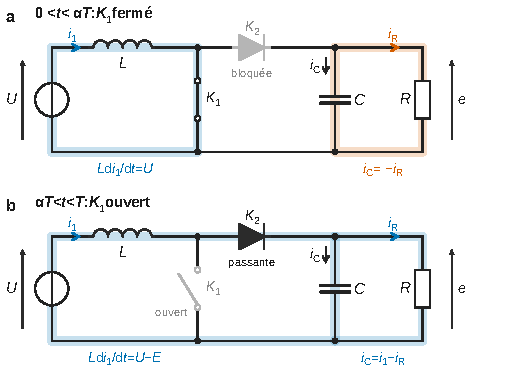
\includegraphics{figures/q18-hacheur-deux-phases.pdf}
\caption*{Figure 2 --- Hacheur parallèle : schémas équivalents avec K1 fermé (a)
puis K1 ouvert (b), chemins de courant surlignés}
\end{figure}

\hypertarget{q19}{%
\subsection{Q19}\label{q19}}

En régime périodique établi, \(i_1(T)=i_1(0)\), donc la tension moyenne aux bornes de la bobine est nulle :
\equationajustee{\alpha T\,U+(1-\alpha)T\,(U-E)=0}
d'où
\equationajustee{\boxed{E=\frac{U}{1-\alpha}}}
On a bien \(E>U\) : c'est un hacheur élévateur. Numériquement, \(\alpha=1-U/E=1-12/30\) :
\equationajustee{\boxed{\alpha=0{,}6}}

\hypertarget{q20}{%
\subsection{Q20}\label{q20}}

\(i_1\) est affine par morceaux :

\begin{itemize}
\tightlist
\item
  il croît de \(I_{1\min}\) à \(I_{1\max}\) avec la pente \(U/L\) pendant \(\alpha T\) ;
\item
  il décroît de \(I_{1\max}\) à \(I_{1\min}\) avec la pente \((U-E)/L\) pendant \((1-\alpha)T\).
\end{itemize}

C'est un \textbf{signal triangulaire} continu, périodique de période \(T\), non symétrique (montée sur \(0{,}6\,T\), descente sur \(0{,}4\,T\)), centré sur sa valeur moyenne \(I_1\), d'ondulation \(\Delta I_1=U\alpha T/L\).

\begin{figure}[H]
\centering
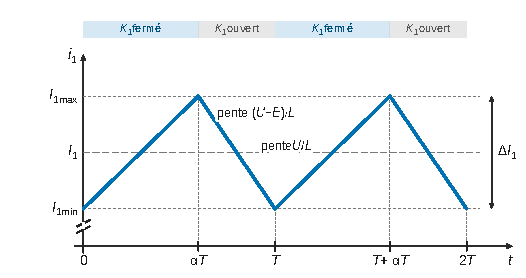
\includegraphics{figures/q20-courant-i1.pdf}
\caption*{Figure 3 --- Allure triangulaire de i1(t) : pente U/L pendant αT, pente
(U − E)/L jusqu'à T, ondulation ΔI1 dilatée}
\end{figure}

Avec \(L=L_{\min}\) (Q22) et \(I_1=12{,}5\) A (Q21) : \(I_{1\max}\simeq13{,}1\) A et \(I_{1\min}\simeq11{,}9\) A.

\hypertarget{q21}{%
\subsection{Q21}\label{q21}}

En régime périodique établi, l'énergie stockée dans \(L\) et \(C\) reprend sa valeur au bout d'une période : leur puissance moyenne est nulle. Les interrupteurs idéaux ne dissipent rien.

La puissance moyenne fournie par la batterie, \(\langle U i_1\rangle=UI_1\) (\(U\) constante), est donc reçue par la charge : \(\langle e\,i_R\rangle\simeq EI_R\) (avec \(e\simeq E\)). Ainsi \(UI_1=EI_R\) et, avec Q19,
\equationajustee{\boxed{I_1=\frac{I_R}{1-\alpha}}}
soit \(I_1=5/0{,}4=12{,}5\) A.

\hypertarget{q22}{%
\subsection{Q22}\label{q22}}

Sur la phase de croissance, \(\Delta I_1=U\alpha T/L\). La contrainte \(\Delta I_1\le0{,}1\,I_1=0{,}1\,I_R/(1-\alpha)\) donne
\equationajustee{L\ge\frac{10\,\alpha(1-\alpha)\,U\,T}{I_R}}
d'où
\equationajustee{\boxed{L_{\min}=\frac{10\,\alpha(1-\alpha)\,UT}{I_R}}}
Application numérique :
\equationajustee{\begin{aligned}
L_{\min}&=\frac{10\times0{,}6\times0{,}4\times12\times50\cdot10^{-6}}{5}\\
&=\frac{1{,}44\cdot10^{-3}}{5}
\end{aligned}}
\equationajustee{\boxed{L_{\min}\simeq2{,}9\cdot10^{-4}\ \mathrm H=0{,}29\ \mathrm{mH}}}

\hypertarget{q23}{%
\subsection{Q23}\label{q23}}

Sur \([0,\alpha T]\), la diode est bloquée (Q18) : \(C\) et \(R\) forment un circuit isolé, avec \(e=u_c\). La loi des nœuds donne \(C\,\dfrac{\mathrm du_c}{\mathrm dt}+\dfrac{u_c}{R}=0\), soit, avec \(\tau=RC\) :
\equationajustee{\boxed{\tau\frac{\mathrm du_c}{\mathrm dt}+u_c=0}}
La solution \(u_c(t)=u_c(0)\,e^{-t/\tau}\) décroît sur \([0,\alpha T]\).

Sur \([\alpha T,T]\), la diode conduit et \(i_C=i_1-i_R\). Comme \(i_1\ge I_{1\min}\simeq11{,}9\ \mathrm A>I_R=5\) A, le condensateur se charge et \(u_c\) croît.

Le maximum de \(u_c\) sur une période est donc atteint en \(T\equiv0\), d'où \(u_c(0)=E_{\max}\) et
\equationajustee{\boxed{u_c(t)=E_{\max}\,e^{-t/\tau}\quad\text{sur }[0,\alpha T]}}

\begin{figure}[H]
\centering
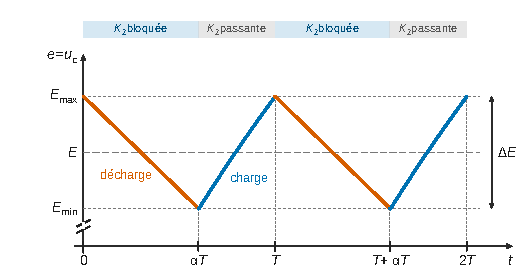
\includegraphics{figures/q23-tension-sortie.pdf}
\caption*{Figure 4 --- Allure de e(t) = uc(t) : décharge de C dans R depuis Emax
quand la diode est bloquée, recharge quand elle conduit}
\end{figure}

\hypertarget{q24}{%
\subsection{Q24}\label{q24}}

\(e\) décroît de \(E_{\max}\) à \(E_{\min}=E_{\max}e^{-\alpha T/\tau}\), donc
\equationajustee{\Delta E=E_{\max}\big(1-e^{-\alpha T/\tau}\big) .}

Approximations :

\begin{enumerate}
\def\labelenumi{\arabic{enumi}.}
\tightlist
\item
  \(\tau\gg T\), donc \(\alpha T/\tau\ll1\) et, par un développement limité à l'ordre 1, \(1-e^{-\alpha T/\tau}\simeq\alpha T/\tau\) ;
\item
  \(\Delta E\ll E\) (100 mV pour 30 V), donc \(E_{\max}\simeq E\).
\end{enumerate}

D'où \(\Delta E\simeq E\alpha T/(RC)\), et la contrainte \(\Delta E\le\Delta E_{\max}\) donne
\equationajustee{\boxed{C_{\min}=\frac{E\,\alpha\,T}{R\,\Delta E_{\max}}}}
Ordre de grandeur, avec \(R=E/I_R=6\ \Omega\) :
\equationajustee{C_{\min}=\frac{30\times0{,}6\times50\cdot10^{-6}}{6\times0{,}1}=1{,}5\cdot10^{-3}\ \mathrm F .}
Alors \(\tau=RC_{\min}=9\) ms \(\gg T=50\ \mu\)s, ce qui valide l'approximation 1.

\hypertarget{partie-iv-blindage-uxe9lectromagnuxe9tique}{%
\section{Partie IV --- Blindage électromagnétique}\label{partie-iv-blindage-uxe9lectromagnuxe9tique}}

\hypertarget{iv.1-moduxe9lisation}{%
\subsection{IV.1 --- Modélisation}\label{iv.1-moduxe9lisation}}

(Pas de question dans cette sous-partie.)

\hypertarget{iv.2-expressions-des-champs-dans-le-conducteur}{%
\subsection{IV.2 --- Expressions des champs dans le conducteur}\label{iv.2-expressions-des-champs-dans-le-conducteur}}

\hypertarget{q25}{%
\subsection{Q25}\label{q25}}

Le conducteur est électriquement neutre (\(\rho=0\)) et assimilable au vide sur le plan diélectrique et magnétique. Les équations de Maxwell s'écrivent :
\equationajustee{\begin{aligned}
\operatorname{div}\vec E&=0\\
\operatorname{div}\vec B&=0\\
\overrightarrow{\mathrm{rot}}\,\vec E&=-\frac{\partial\vec B}{\partial t}\\
\overrightarrow{\mathrm{rot}}\,\vec B&=\mu_0\vec\jmath+\mu_0\varepsilon_0\frac{\partial\vec E}{\partial t}
\end{aligned}}
et la loi d'Ohm locale
\equationajustee{\boxed{\vec\jmath=\gamma\,\vec E}}

\hypertarget{q26}{%
\subsection{Q26}\label{q26}}

En régime sinusoïdal, le rapport des deux termes de Maxwell-Ampère vaut :
\equationajustee{\frac{\big\|\varepsilon_0\,\partial\vec E/\partial t\big\|}{\|\gamma\vec E\|}=\frac{\varepsilon_0\omega}{\gamma} .}
Pour le cuivre, \(\gamma=1/(17\cdot10^{-9})\simeq6\cdot10^7\ \mathrm{S\cdot m^{-1}}\). Pour \(f\le10\) GHz :
\equationajustee{\frac{\varepsilon_0\omega}{\gamma}\le\frac{2\pi\times8{,}85\cdot10^{-12}\times10^{10}}{6\cdot10^{7}}\sim10^{-8}\ll1 .}
Même pour le métal le moins conducteur du tableau (zinc, \(\gamma\simeq1{,}6\cdot10^7\ \mathrm{S\cdot m^{-1}}\)), le rapport reste de l'ordre de \(3\cdot10^{-8}\). Le courant de déplacement est négligeable :
\equationajustee{\boxed{\overrightarrow{\mathrm{rot}}\,\vec B=\mu_0\vec\jmath=\mu_0\gamma\vec E}}

\hypertarget{q27}{%
\subsection{Q27}\label{q27}}

On prend le rotationnel de Maxwell-Faraday, en permutant les dérivées spatiales et temporelles :
\equationajustee{\begin{aligned}
\overrightarrow{\mathrm{rot}}\big(\overrightarrow{\mathrm{rot}}\,\vec E\big)&=-\frac{\partial}{\partial t}\overrightarrow{\mathrm{rot}}\,\vec B\\
&=-\mu_0\gamma\frac{\partial\vec E}{\partial t}
\end{aligned}}
D'après la formule fournie et \(\operatorname{div}\vec E=0\) (neutralité), le membre de gauche vaut \(-\Delta\vec E\) :
\equationajustee{\boxed{\Delta\vec E-\mu_0\gamma\frac{\partial\vec E}{\partial t}=\vec 0}}
soit \(\boxed{\alpha=\mu_0\gamma}\).

\hypertarget{q28}{%
\subsection{Q28}\label{q28}}

Par homogénéité, \([\alpha]=[\Delta\vec E]/[\partial_t\vec E]=\mathrm{s\cdot m^{-2}}\) (et \(\mu_0\gamma\) en \(\mathrm{H\cdot S\cdot m^{-2}}=\mathrm{s\cdot m^{-2}}\)) :
\equationajustee{\boxed{\alpha\ \text{en}\ \mathrm{s\cdot m^{-2}}}}
Premier ordre en temps, second ordre en espace : c'est une \textbf{équation de diffusion} (phénomène irréversible), de coefficient de diffusion \(1/(\mu_0\gamma)\), et non une équation de d'Alembert (second ordre en temps). On la rencontre en \textbf{diffusion thermique} (loi de Fourier) et en \textbf{diffusion de particules} (loi de Fick, partie I).

\hypertarget{q29}{%
\subsection{Q29}\label{q29}}

Pour \(\underline{\vec E}=E_0e^{j(\omega t-\underline kz)}\vec e_x\), on a \(\Delta\to-\underline k^2\) et \(\partial_t\to j\omega\), d'où
\equationajustee{\boxed{\underline k^2=-j\,\mu_0\gamma\,\omega}}
Avec \(\mu_0\gamma\omega=2/\delta^2\) et \(-2j=(1-j)^2\), on obtient \(\underline k=\pm(1-j)/\delta\). On retient \(\underline k=(1-j)/\delta\), pour laquelle \(e^{-j\underline kz}=e^{-z/\delta}e^{-jz/\delta}\) décroît dans le conducteur (\(z>0\)) ; l'autre racine divergerait.

La partie réelle du vecteur d'onde,
\equationajustee{\mathrm{Re}(\underline k)=\frac1\delta=\sqrt{\frac{\mu_0\gamma\omega}{2}},}
n'est pas proportionnelle à \(\omega\) (elle varie comme \(\sqrt\omega\)). La vitesse de phase \(v_\varphi=\omega/\mathrm{Re}(\underline k)=\sqrt{2\omega/(\mu_0\gamma)}\) dépend donc de \(\omega\) : \textbf{le conducteur ohmique est un milieu dispersif} (et absorbant, puisque \(\underline k\) a une partie imaginaire).

\hypertarget{q30}{%
\subsection{Q30}\label{q30}}

Avec \(-j\underline kz=-z/\delta-jz/\delta\) :
\equationajustee{\boxed{\underline{\vec E}=E_0\,e^{-z/\delta}\,e^{j(\omega t-z/\delta)}\,\vec e_x}}
et, par la loi d'Ohm locale :
\equationajustee{\boxed{\underline{\vec\jmath}=\gamma E_0\,e^{-z/\delta}\,e^{j(\omega t-z/\delta)}\,\vec e_x}}
En réel : \(\vec E=E_0e^{-z/\delta}\cos(\omega t-z/\delta)\,\vec e_x\), et \(\vec\jmath\) est en phase avec \(\vec E\).

\hypertarget{q31}{%
\subsection{Q31}\label{q31}}

\(\delta=\sqrt{2/(\mu_0\gamma\omega)}\) est l'\textbf{épaisseur de peau}, une longueur exprimée \textbf{en mètres} (on vérifie : \(\mu_0\gamma\omega\) est en \(\mathrm{m^{-2}}\) d'après Q28).

Pour \(z\gg\delta\), le facteur \(e^{-z/\delta}\) rend \(\vec E\) et \(\vec B\) (et \(\vec\jmath\)) \textbf{pratiquement nuls}.

Les champs sont confinés dans une couche superficielle d'épaisseur de quelques \(\delta\) (effet de peau). À \(z=5\delta\), l'amplitude est déjà divisée par \(e^5\simeq150\).

\begin{figure}[H]
\centering
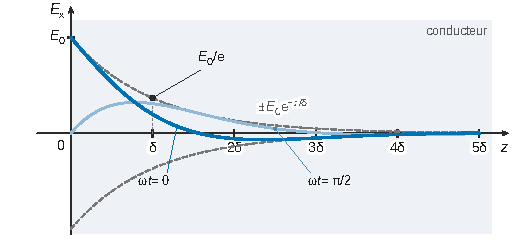
\includegraphics{figures/q31-effet-peau.pdf}
\caption*{Figure 5 --- Effet de peau : champ Ex(z) à deux instants sous
l'enveloppe ±E0 exp(−z/δ)}
\end{figure}

Remarque : Maxwell-Faraday donne
\equationajustee{\underline B_y=\frac{\underline k\,\underline E_x}{\omega}=\frac{\sqrt2E_0}{\delta\omega}e^{-z/\delta}e^{j(\omega t-z/\delta-\pi/4)} .}
Le module coïncide avec l'expression admise, mais le déphasage est \(-\pi/4\) et non \(+\pi/4\) comme l'écrit l'énoncé. Ce signe n'a pas d'effet sur les valeurs moyennes de Q34 (qui font intervenir \(\cos(\pi/4)\), fonction paire). On garde l'expression de l'énoncé.

\hypertarget{iv.3-considuxe9rations-physiques-sur-luxe9crantage}{%
\subsection{IV.3 --- Considérations physiques sur l'écrantage}\label{iv.3-considuxe9rations-physiques-sur-luxe9crantage}}

\hypertarget{q32}{%
\subsection{Q32}\label{q32}}

\(\delta=1/\sqrt{\pi\mu_0\gamma f}\) décroît quand \(f\) croît. À épaisseur de dépôt donnée, l'atténuation est d'autant plus forte que la fréquence est élevée : \textbf{l'écrantage est plus efficace en haute fréquence}.

À \(f=1\) MHz, pour le cuivre (\(\gamma\simeq6\cdot10^7\ \mathrm{S\cdot m^{-1}}\), \(\omega\simeq6{,}3\cdot10^6\) rad/s) :
\equationajustee{\mu_0\gamma\omega\simeq1{,}26\cdot10^{-6}\times6\cdot10^7\times6{,}3\cdot10^6\simeq4{,}7\cdot10^8\ \mathrm{m^{-2}}}
d'où
\equationajustee{\delta=\sqrt{\frac{2}{4{,}7\cdot10^8}}\simeq6{,}5\cdot10^{-5}\ \mathrm m .}
Une épaisseur de \(3\delta\) à \(5\delta\) atténue l'amplitude d'un facteur 20 à 150 :
\equationajustee{\boxed{e_{\text{\text{dépôt}}}\sim0{,}2\ \text{\text{à}}\ 0{,}3\ \mathrm{mm}}}
Les autres métaux du tableau donnent le même ordre de grandeur (\(\delta\) de 64 µm pour l'argent à 124 µm pour le zinc).

\hypertarget{q33}{%
\subsection{Q33}\label{q33}}

Le champ électrique met en mouvement les porteurs libres : il crée des courants induits \(\vec\jmath=\gamma\vec E\) qui dissipent l'énergie de l'onde par \textbf{effet Joule} (puissance volumique \(\vec\jmath\cdot\vec E=\gamma E^2>0\)). Cette dissipation explique l'atténuation de l'onde dans le conducteur.

\hypertarget{q34}{%
\subsection{Q34}\label{q34}}

Champs réels, avec \(\theta=\omega t-z/\delta\) :
\equationajustee{\begin{aligned}
\vec E&=E_0e^{-z/\delta}\cos\theta\,\vec e_x\\
\vec B&=\frac{\sqrt2E_0}{\delta\omega}e^{-z/\delta}\cos\!\Big(\theta+\frac\pi4\Big)\vec e_y
\end{aligned}}
Vecteur de Poynting :
\equationajustee{\vec\Pi=\frac{\vec E\wedge\vec B}{\mu_0}=\frac{\sqrt2E_0^2}{\mu_0\delta\omega}e^{-2z/\delta}\cos\theta\cos\!\Big(\theta+\frac\pi4\Big)\vec e_z .}
D'après la formule de linéarisation, \(\big\langle\cos\theta\cos(\theta+\frac\pi4)\big\rangle=\frac12\cos\frac\pi4=\frac{\sqrt2}4\), donc
\equationajustee{\langle\vec\Pi\rangle=\frac{E_0^2}{2\mu_0\delta\omega}e^{-2z/\delta}\,\vec e_z .}
Puissance moyenne entrant à travers \(S\) en \(z=0^+\), avec \(1/\delta=\sqrt{\mu_0\gamma\omega/2}\) :
\equationajustee{\begin{aligned}
\mathcal P_{\text{ent}}&=\frac{E_0^2S}{2\mu_0\delta\omega}\\
&=\frac{E_0^2S}{2}\sqrt{\frac{\gamma}{2\mu_0\omega}}
\end{aligned}}
\equationajustee{\boxed{\mathcal P_{\text{ent}}=\frac{\sqrt2}{4}E_0^2S\sqrt{\frac{\gamma}{\mu_0\omega}}}}

\hypertarget{q35}{%
\subsection{Q35}\label{q35}}

Puissance volumique dissipée : \(\vec\jmath\cdot\vec E=\gamma E^2=\gamma E_0^2e^{-2z/\delta}\cos^2\theta\), de moyenne \(\frac{\gamma E_0^2}{2}e^{-2z/\delta}\). Sur le volume \(S\,\mathrm dz\) :
\equationajustee{\boxed{\mathrm d\mathcal P_J=\frac{\gamma E_0^2S}{2}\,e^{-2z/\delta}\,\mathrm dz}}

\hypertarget{q36}{%
\subsection{Q36}\label{q36}}

\equationajustee{\begin{aligned}
\mathcal P_J&=\int_0^{+\infty}\frac{\gamma E_0^2S}{2}e^{-2z/\delta}\,\mathrm dz\\
&=\frac{\gamma E_0^2S\delta}{4}\\
&=\frac{\gamma E_0^2S}{4}\sqrt{\frac{2}{\mu_0\gamma\omega}}
\end{aligned}}
\equationajustee{\boxed{\mathcal P_J=\frac{\sqrt2}{4}E_0^2S\sqrt{\frac{\gamma}{\mu_0\omega}}}}
\textbf{Conclusion} : \(\mathcal P_J=\mathcal P_{\text{ent}}\). Toute la puissance qui pénètre dans le conducteur y est dissipée par effet Joule, sans rien transmettre en profondeur. Cela confirme la réponse de Q33 : l'atténuation est due à l'effet Joule.

\end{document}
